% !TEX encoding = MacOSRoman
\documentclass[12pt,a4paper,english]{article}

% Note that you must choose either Finnish or English here and there in this
% file.
% Other options for document class
  % ,twoside,openright   % If printing on both sides (>80 pages)
  % ,twocolumn           % Can be used in lab reports, not in theses

% Ensure the correct Pdf size (not needed in all environments)
\special{papersize=210mm,297mm}

\usepackage[utf8]{inputenc}
\usepackage[T1]{fontenc}
\usepackage{hyperref}
\usepackage{amsfonts}
\usepackage{textcomp}
\usepackage{listings}
\usepackage{graphicx}
\usepackage{numprint}
\usepackage{subfigure}
\usepackage{tikz}
\usetikzlibrary{shapes.geometric, arrows}
\usepackage{setspace}
%\usepackage{termlist}
\usepackage{amsmath}
\usepackage{amssymb}
\usepackage{amsthm}
\usepackage{bm}

%new commands
\newcommand\todo[1]{{\color{red}!!!TODO: #1}}
\DeclareMathOperator{\tr}{\mathrm{tr}}

\author{Jordi Anguera\thanks{Autonomous University of Barcelona, Spain} \and Leevi Annala\thanks{University of Jyväskylä, Finland} \and Stefan Dimitrijevic\thanks{University of Novi Sad, Serbia} \and Patricia Pauli\thanks{Technical University of Darmstadt, Germany} \and Liisa-Ida Sorsa\thanks{Tampere University of Technology, Finland} \and Dimitar Trendafilov\thanks{University of Sofia ''St. Kliment Ohridski'', Bulgaria} \and Christophe Pickard\thanks{University of Grenoble Alpes and Grenoble INP, France}}
\title{Modeling effect of time delay for large network of seismic monitor} 
\date{17.7.2018}

\begin{document}
\maketitle

\begin{abstract}

\end{abstract}

\section{Introduction}

The purpose of this work is to analyze noise in a large network of seismic monitors and to extract clock drift from the noise. 

\section{Data}

The data is collected from a network of 73 seismic monitor stations recording ground vibrations in the Southeast region of France. The GPS coordinate position of each station in the network is known (Figure \ref{fig:monitornetwork}) and they each contain a clock which is synchronized to the GPS once a month. The seismic monitor sensor records compression and decompression as discrete values -1 and 1, respectively, every second. The sensor responds to any event in the area, be it an earthquake, tremor from road traffic, airplane or any other pressure wave which travels in the ground.

\begin{figure}[ht]
  \begin{center}   
   \includegraphics[width=\textwidth]{InitialStationSet.png}
  \end{center}
  \caption{The network of seismic monitors are located in the Southeast France, mostly in the regions of Provence-Alpes-C\^{o}te d'Azur and Rh\^{o}ne-Alpes. The seven stations chosen as the small test set is shown as green in the southeast part of the area.}\label{fig:monitornetwork}
\end{figure}

The stations work independent of each other and are occasionally shut down for some time frame for maintenance, repair or just random events. Just as occasionally they are brought up to measure again. Therefore, the number of active stations varies over time. The Figure \ref{fig:workingstations} shows the number of working stations, and the Figure \ref{fig:workingconnections} the number of working connections between the monitor stations over one year of measurements. 

\begin{figure*}[ht] 
  \centering 
\subfigure[The number of working seismic monitor stations.]{\label{fig:workingstations}\includegraphics[width=0.48\linewidth]{working_connections.png}}
\subfigure[The number of working connections between the stations.]{\label{fig:workingconnections}\includegraphics[width=0.48\linewidth]{working_connections.png}}
\caption{Working stations and connections over one year time period. \todo{update figures here}}
\label{fig:workingmonitors}
\end{figure*}

The compression and decompression data recorded by the stations is retrieved and run through initial data cleaning and filtering procedures. The data is then cross-correlated in one-hour time windows to yield time-delay data of signal between each monitor (Figure \ref{fig:examplesignal}). 

\begin{figure}[ht]
  \begin{center}   
   \includegraphics[width=0.7\textwidth]{delayevolutionovertimeforonestation2.png}
  \end{center}
  \caption{The time-delay signal recorded by one station over a year. The time delay is computed in one-hour windows, yielding 24 time-delay values over a day.}\label{fig:examplesignal}
\end{figure}

The time delays between each monitor are assumed to depend on the distance between the monitor. The further away the monitors are from each other, the larger the time delay caused by the same event recorded by the monitor. The Figure \ref{fig:histograms} shows an example of time-delay evolution of one monitor station over 24 hours. The distributions  are symmetric because each monitor connection is computed into both directions. The interesting feature of the histograms is how the shape of the distribution changes. 

\begin{figure}[ht]
  \begin{center}   
   \includegraphics[width=\textwidth]{hourlydelaydistributionoverallstationsforoneday.png}
  \end{center}
  \caption{Histograms of time-delays recorded by one station over 24 hours. The figure shows clearly how the time-delays between detected events change over time.}\label{fig:histograms}
\end{figure}

\section{Methods}

\subsection{Modelling time delay between seismic monitors}
The network of monitors can be modelled as a complete graph. The signal of each monitor is cross-correlated with other monitor signals, finally yielding time-delay data between each monitor. The time delay between the monitors comprise information on the real time the signal travels between the monitors, the inaccuracies of the clock (time drift), and other noise affecting the measurement. 

Let $\bm{\hat{\delta}} \in \mathbb{R}^{n\times n}$ be the measured pairwise time delays of the system, $\bm{\delta}$ the actual pairwise time delays, and $\bm{\varepsilon}$ an error term including clock drift of the station's clock and other errors

\begin{equation}
\bm{\hat{\delta}}  = \bm{\delta} + \bm{\varepsilon}.
\label{eq:model}
\end{equation}
 
Each of the monitors are equipped with a clock which runs independent of others. It is synchronized via GPS system once a month and then runs independently. The drift, $\varepsilon_i$ in clock $i$ is caused by variation in the clocks oscillator.  

The position of each seismic monitor in the network is known. As the monitors are spread across a large area, it is assumed that local tremors are detected by stations that are close by, and therefore the correlations found in the pairwise cross-correlations and time delay data between them have higher likelihood to be linked. 

\subsection{Denoising model}
\subsubsection{Definitions}
The computational denoising model involves weighted network estimation by the use of topological graph metrics, described in detail in \cite{Spyrou2017}. 

We have a weighted graph $\mathcal{G} = (\mathcal{V}, \mathcal{E}, \bf{\hat{\delta}}_t)$ defined by a finite set of nodes $\mathcal{V}$ with $|\mathcal{V}| = n$, a set of edges $\mathcal{E} = \{ (v_i,v_j) \in \mathcal{E} \}$, with $|\mathcal{E}| = n^2-n$ and the weighted adjacency matrix $\bm{\hat{\delta}}$ with $\delta_{ii} = 0$ for all $i$. The matrix $\bm{\hat{\delta}}$  is symmetric and describes the time delays between events in the graph, and is normalized, i.e. $\hat{\delta}_{ij}\in [0,1]$. The adjacency matrix indicates the strength of connection between nodes. Therefore, the shorter the time delay between nodes, the stronger the connection, and higher the value. 

\subsubsection{Cost function}
We assume to have estimates of $M$ differentiable graph metrics of the original matrix $\bm{\delta}$, i.e. $f_m(\bm{\delta}) = K_m$, where $m\in\{ 1,\dots, M \}$, then we can formulate a cost function that measures the deviation of the observed weight matrix's metrics $f_m(\bm{\hat{\delta}})$ to the estimates $K_m$ as: 

\begin{equation}
c(\bm{\hat{\delta}}) = \sum_m e_m^2(\bm{\hat{\delta}}) = \sum_m(f_m(\bm{\hat{\delta}})-K_m)^2
\end{equation}

The error is minimized with gradient descent updates on $\bm{\hat{\delta}}$: 

\begin{equation}
\bm{\hat{\delta}}^{(t+1)} = \bm{\hat{\delta}}^t-\mu\sum_m e_m(\bm{\hat{\delta}}^t)\frac{df_m(\bm{\hat{\delta}}^t)}{d\bm{\hat{\delta}}^t},
\label{eq:updates}
\end{equation}

where $t$ is the iteration index and $\mu$ the learning rate. For the case of $m=1$, Equation \ref{eq:updates} describes the traditional single function gradient descent. 

\subsubsection{Graph metrics}
Graph metrics are scalar functions of the weight matrix, $f(\bm{\hat{\delta}}): \mathbb{R}^{n \times n}\rightarrow \mathbb{R}$. We choose graph metrics to:
\begin{enumerate}
\item \textbf{Distance}: We want to use the distance measures to denoise the delay measurements. For this purpose, we deisigned a metric, the connection strength of a node i. We normalize the delays and compute the row sum 

\begin{equation}
f_i (\bm{\delta})= \sum_j{\delta_{ij}}.  
\end{equation}

Thde connection strength can be interpreted as the sum of all normalized delays of all of the links to node i.

\begin{figure}[htb]
\centering
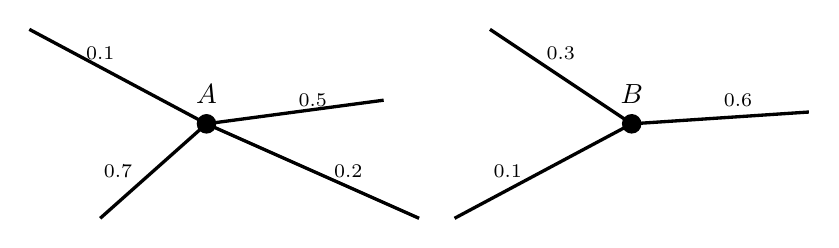
\begin{tikzpicture}[xscale=0.45, yscale=0.3]
\begin{scope}[shift={(0,2)}]
\draw [-,very thick] (5,0) -- (8,4);
\draw [-,very thick] (14,0) -- (8,4);
\draw [-,very thick] (8,4) -- (13,5);
\draw [-,very thick] (8,4) -- (3,8);
\node[circle,fill,inner sep=2.5pt, label=above:$A$] at (8,4) {} ;
\node [align=center] at (11,5) {\scriptsize 0.5};
\node [align=center] at (5,7) {\scriptsize 0.1};
\node [align=center] at (5.5,2) {\scriptsize 0.7};
\node [align=center] at (12,2) {\scriptsize 0.2};
\draw [-,very thick] (15,0) -- (20,4);
\draw [-,very thick] (20,4) -- (25,4.5);
\draw [-,very thick] (20,4) -- (16,8);
\node[circle,fill,inner sep=2.5pt, label=above:$B$] at (20,4) {} ;
\node [align=center] at (18,7) {\scriptsize 0.3};
\node [align=center] at (16.5,2) {\scriptsize 0.1};
\node [align=center] at (23,5) {\scriptsize 0.6};


\end{scope}
\end{tikzpicture}
\caption{Distance metric.} \label{fig:1}
\end{figure}
Figure \ref{fig:1} shows two nodes. Node $A$ has four connections yielding a connection strength $0.1+0.5+0.7+0.6=1.9$ whereas node $B$ only has three connections. Thus, the connection strength is $0.3+0.6+0.1=1$.



The constants $K_m$ are defined as follows
\begin{equation}
K_m=f_m(\bm W_d)
\end{equation}
It is the connection strength as well. But now we plug in the distance matrix $\bm{W_d}$. The distances are constants and yield a constant $K_m$.
The weight matrix $\bm{W_d}$ is a function of the distance between node $i$ and node $j$. First, we choose the function to be the reciprocal of the distances of the node to all other nodes, $d _{ij}= 1/r_{ij}$, normalized between $[0,1]$. Higher values correspond to nodes with short distances to all other nodes. Second, we try a metric with weights proportional to the distances, normailzed between $[0,1]$ accordingly. Here, high values correspond to long distances between two stations.

We find the derivative for the gradient descent update step.
\begin{equation}
\frac{df_2}{d\bm{\delta}}=\frac{\sum_j\delta_{ij}}{d\bm{\delta}}=
\begin{bmatrix}
    0 & 1 & 0 & \dots  & 0 \\
    1 & 0 & 1 & \dots  & 1 \\
    \vdots & \vdots & \vdots & \ddots & \vdots \\
    0 & 1 & 0 & \dots  & 0
\end{bmatrix}
\end{equation}
It is a symmetric matrix with ones in the ith row and ith column. The diagonal entries remain zero.


We expect the following correlation between the distance of two stations and the delay between them. The further apart the stations, the greater is the delay. Figure \ref{fig:nearfar} shows that the variance of the delays is much higher for a station pair of stations that are far apart.

\begin{figure}[ht]
  \begin{center}   
   \includegraphics[width=\textwidth]{Comparisondelayoverrandomdayoffarestandclosestlinks.png}
  \end{center}
  \caption{Comparison of the Delay of the Farest and Closest Station Pairs over a Random Day.}\label{fig:nearfar}
\end{figure}


 
\item Average neighbour degree, resilience: 

The average neighbour degree for node $i$ is given by

\end{enumerate}




%% Insert bibliography
\bibliographystyle{abbrv}  
\bibliography{references}   

\end{document}
